\documentclass[crop,tikz,convert={outext=.svg,command=\unexpanded{pdf2svg \infile\space\outfile}},multi=false]{standalone}
%\usetikzlibrary{...}% tikz package already loaded by 'tikz' option
\usepackage{amsmath,amssymb,amsthm,bm}
\usepackage{xcolor}
\definecolor{Solarized-base03}{RGB}{0, 43, 54}
\definecolor{Solarized-base02}{RGB}{7, 54, 66}
\definecolor{Solarized-base01}{RGB}{88, 110, 117}
\definecolor{Solarized-base00}{RGB}{101, 123, 131}
\definecolor{Solarized-base0}{RGB}{131, 148, 150}
\definecolor{Solarized-base1}{RGB}{147, 161, 161}
\definecolor{Solarized-base2}{RGB}{238, 232, 213}
\definecolor{Solarized-base3}{RGB}{253, 246, 227}
\definecolor{Solarized-yellow}{RGB}{181, 137, 0}
\definecolor{Solarized-orange}{RGB}{203, 75, 22}
\definecolor{Solarized-red}{RGB}{220, 50, 47}
\definecolor{Solarized-magenta}{RGB}{211, 54, 130}
\definecolor{Solarized-violet}{RGB}{108, 113, 196}
\definecolor{Solarized-blue}{RGB}{38, 139, 210}
\definecolor{Solarized-cyan}{RGB}{42, 161, 152}
\definecolor{Solarized-green}{RGB}{133, 153, 0}
\color{Solarized-base02}
\pagecolor{Solarized-base3}
\everymath{\color{Solarized-magenta}}
\usepackage{ifthen}
\usetikzlibrary{backgrounds,automata,shapes,snakes,arrows,arrows.meta,chains,positioning,calc}
\def \av {\bm{a}}
\def \bv {\bm{b}}
\def \cv {\bm{c}}
\def \dv {\bm{d}}
\def \ev {\bm{e}}
\def \fv {\bm{f}}
\def \gv {\bm{g}}
\def \hv {\bm{h}}
\def \kv {\bm{k}}
\def \pv {\bm{p}}
\def \qv {\bm{q}}
\def \tv {\bm{t}}
\def \uv {\bm{u}}
\def \vv {\bm{v}}
\def \wv {\bm{w}}
\def \xv {\bm{x}}
\def \yv {\bm{y}}
\def \zv {\bm{z}}
\def \Av {\mathbf{A}}
\def \Bv {\mathbf{B}}
\def \Cv {\mathbf{C}}
\def \Dv {\mathbf{D}}
\def \Fv {\mathbf{F}}
\def \Gv {\mathbf{G}}
\def \Hv {\mathbf{H}}
\def \Iv {\mathbf{I}}
\def \Kv {\mathbf{K}}
\def \Lv {\mathbf{L}}
\def \Mv {\mathbf{M}}
\def \Pv {\mathbf{P}}
\def \Qv {\mathbf{Q}}
\def \Sv {\mathbf{S}}
\def \Uv {\mathbf{U}}
\def \Vv {\mathbf{V}}
\def \Wv {\mathbf{W}}
\def \Xv {\mathbf{X}}
\def \Yv {\mathbf{Y}}
\def \Zv {\mathbf{Z}}
\makeatletter
\begin{document}
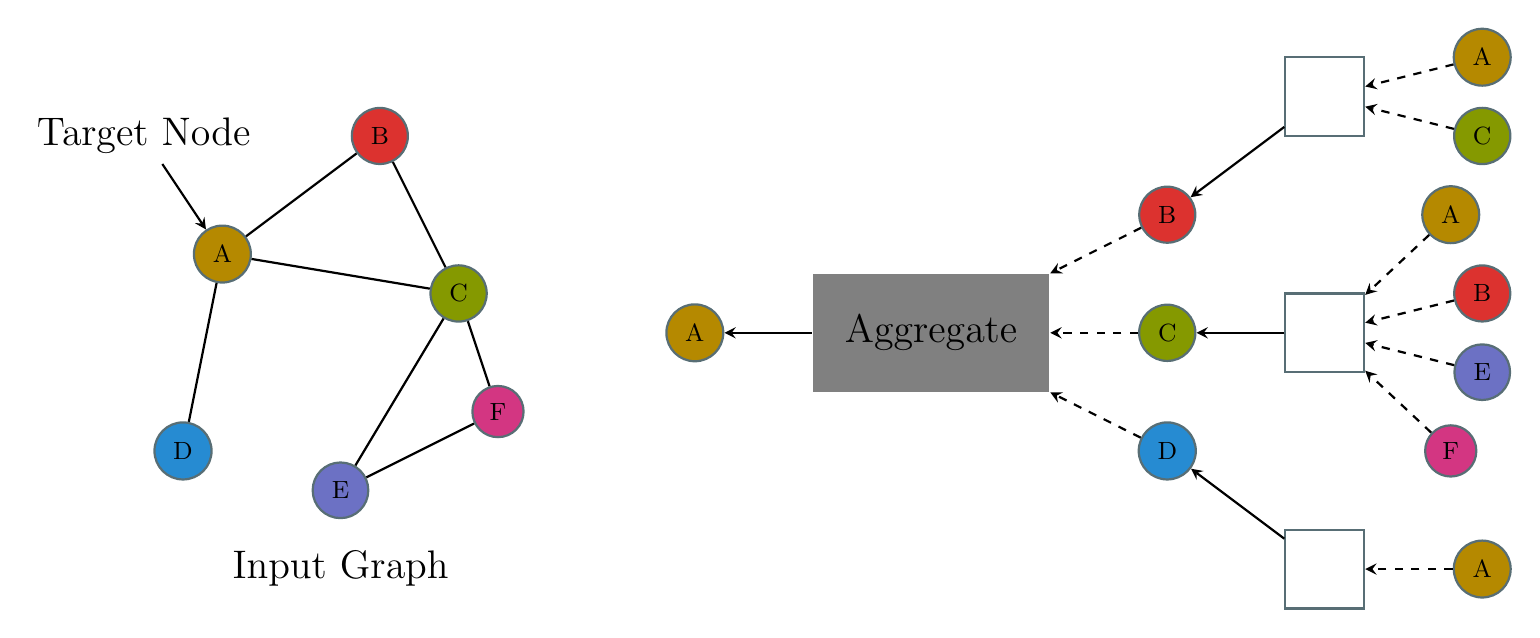
\begin{tikzpicture} [ % 先定义每类点的样式
    thick, >=stealth, scale=1, font=\small,
    rec/.style = {shape = rectangle,minimum height = 1.5cm, minimum width = 3cm, align = center, fill = gray, font = \fontsize{14}{4}\selectfont},
    rec2/.style = {shape = rectangle,minimum height = 1cm, minimum width = 1cm, align = center, draw=Solarized-base01, font = \fontsize{18}{4}\selectfont},
    rec3/.style = {shape = rectangle, align = center, font = \fontsize{14}{4}\selectfont},
    point-A/.style = {circle, inner sep=4.0pt, fill=Solarized-yellow, draw=Solarized-base01},
    point-B/.style = {circle, inner sep=4.0pt, fill=Solarized-red, draw=Solarized-base01},
    point-C/.style = {circle, inner sep=4.0pt, fill=Solarized-green, draw=Solarized-base01},
    point-D/.style = {circle, inner sep=4.0pt, fill=Solarized-blue, draw=Solarized-base01},
    point-E/.style = {circle, inner sep=4.0pt, fill=Solarized-violet, draw=Solarized-base01},
    point-F/.style = {circle, inner sep=3.5pt, fill=Solarized-magenta, draw=Solarized-base01}
]

% \draw [help lines, step = 1] (-10,-10) grid (10,10);
% \filldraw (0,0) circle (0.1);

% 中间矩形
\node [rec] (r) at (-0.5,0){Aggregate};
\node [point-A] (pla1) at (-3.5,0){A};

\node [rec3] (tex) at (-10.5,2.5){Target Node};
\node [rec3] (tex2) at (-8,-3){Input Graph};

% 右边点
\node [point-A] (pra1) at (6.5,3.5){A};
\node [point-C] (prc1) at (6.5,2.5){C};
\node [point-A] (pra2) at (6.1,1.5){A};
\node [point-B] (prb1) at (6.5,0.5){B};
\node [point-E] (pre1) at (6.5,-0.5){E};
\node [point-F] (prf1) at (6.1,-1.5){F};
\node [point-A] (pra3) at (6.5,-3){A};

% 右边中间
\node [point-B] (prcb) at (2.5,1.5){B};
\node [point-C] (prcc) at (2.5,0){C};
\node [point-D] (prcd) at (2.5,-1.5){D};

% 正方形
\node [rec2] (rr1) at (4.5,3){};
\node [rec2] (rr2) at (4.5,0){};
\node [rec2] (rr3) at (4.5,-3){};

% 左边点
\node [point-F] (plf) at (-6,-1){F};
\node [point-C] (plc) at (-6.5,0.5){C};
\node [point-B] (plb) at (-7.5,2.5){B};
\node [point-A] (pla) at (-9.5,1){A};
\node [point-D] (pld) at (-10,-1.5){D};
\node [point-E] (ple) at (-8,-2){E};

% 连线
\draw (pla)--(plb)--(plc)--(plf)--(ple)--(plc)--(pla)--(pld);

\draw [thick,->](r)--(pla1);
\draw [thick,->](rr1)--(prcb);
\draw [thick,->](rr2)--(prcc);
\draw [thick,->](rr3)--(prcd);

\draw [thick,->](tex)--(pla);

\draw [dashed,->](prcb)--(r);
\draw [dashed,->](prcc)--(r);
\draw [dashed,->](prcd)--(r);

\draw [dashed,->](pra1)--(rr1);
\draw [dashed,->](prc1)--(rr1);

\draw [dashed,->](pra2)--(rr2);
\draw [dashed,->](prb1)--(rr2);
\draw [dashed,->](pre1)--(rr2);
\draw [dashed,->](prf1)--(rr2);

\draw [dashed,->](pra3)--(rr3);

\end{tikzpicture}


\end{document}